\documentclass[14pt]{extbook}
\usepackage{multicol, enumerate, enumitem, hyperref, color, soul, setspace, parskip, fancyhdr} %General Packages
\usepackage{amssymb, amsthm, amsmath, bbm, latexsym, units, mathtools} %Math Packages
\everymath{\displaystyle} %All math in Display Style
% Packages with additional options
\usepackage[headsep=0.5cm,headheight=12pt, left=1 in,right= 1 in,top= 1 in,bottom= 1 in]{geometry}
\usepackage[usenames,dvipsnames]{xcolor}
\usepackage{dashrule}  % Package to use the command below to create lines between items
\newcommand{\litem}[1]{\item#1\hspace*{-1cm}\rule{\textwidth}{0.4pt}}
\pagestyle{fancy}
\lhead{Progress Quiz 3}
\chead{}
\rhead{Version C}
\lfoot{}
\cfoot{}
\rfoot{Fall 2020}
\begin{document}

\begin{enumerate}
\litem{
What is the domain of the function below?\[ f(x) = \sqrt[4]{8 x + 7} \]\begin{enumerate}[label=\Alph*.]
\item \( (-\infty, a], \text{where } a \in [-1.04, -0.82] \)
\item \( (-\infty, \infty) \)
\item \( [a, \infty), \text{where } a \in [-1.28, -1.01] \)
\item \( [a, \infty), \text{ where } a \in [-0.9, -0.84] \)
\item \( (-\infty, a], \text{where } a \in [-1.45, -1.08] \)

\end{enumerate} }
\litem{
Solve the radical equation below. Then, choose the interval(s) that the solution(s) belongs to.\[ \sqrt{5 x + 4} - \sqrt{-8 x - 7} = 0 \]\begin{enumerate}[label=\Alph*.]
\item \( x \in [-0.87,-0.81] \)
\item \( x_1 \in [-0.87, -0.81] \text{ and } x_2 \in [-0.8,1.2] \)
\item \( x \in [0.17,0.28] \)
\item \( \text{All solutions lead to invalid or complex values in the equation.} \)
\item \( x_1 \in [-0.91, -0.85] \text{ and } x_2 \in [-0.8,1.2] \)

\end{enumerate} }
\litem{
Choose the graph of the equation below.\[ f(x) = - \sqrt{x - 6} + 7 \]\begin{enumerate}[label=\Alph*.]
\begin{multicols}{2}\item 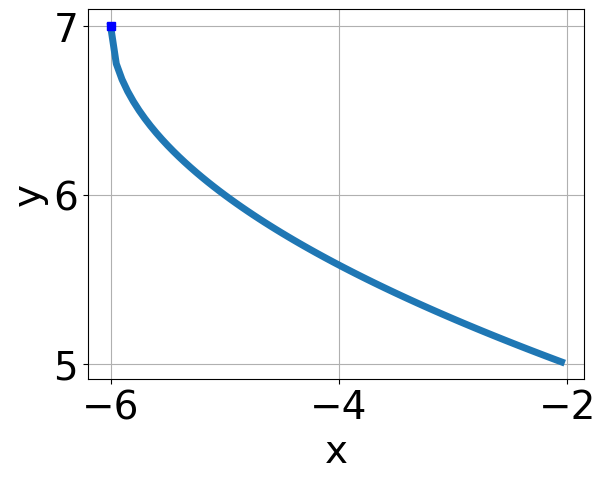
\includegraphics[width = 0.3\textwidth]{../Figures/radicalEquationToGraphAC.png}\item 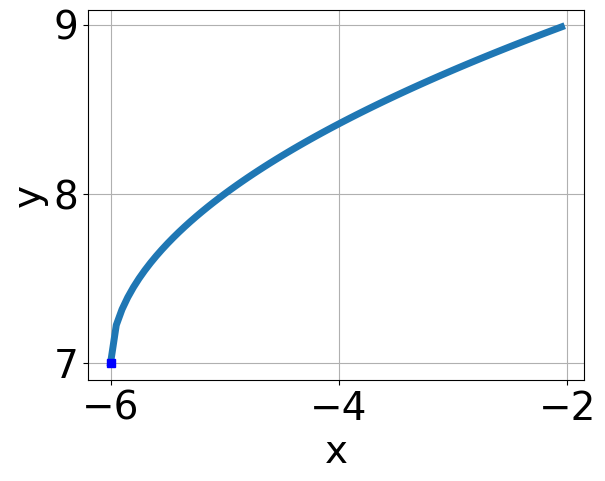
\includegraphics[width = 0.3\textwidth]{../Figures/radicalEquationToGraphBC.png}\item 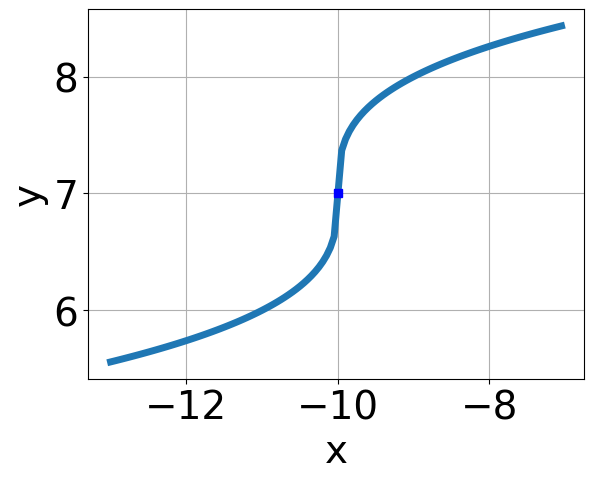
\includegraphics[width = 0.3\textwidth]{../Figures/radicalEquationToGraphCC.png}\item 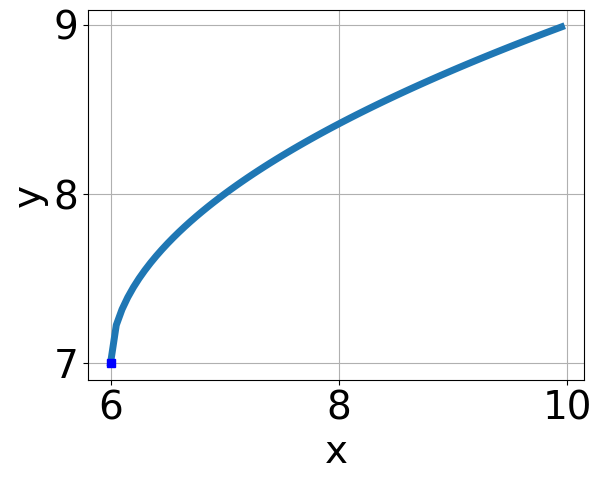
\includegraphics[width = 0.3\textwidth]{../Figures/radicalEquationToGraphDC.png}\end{multicols}\item None of the above.
\end{enumerate} }
\litem{
Choose the equation of the function graphed below.
\begin{center}
    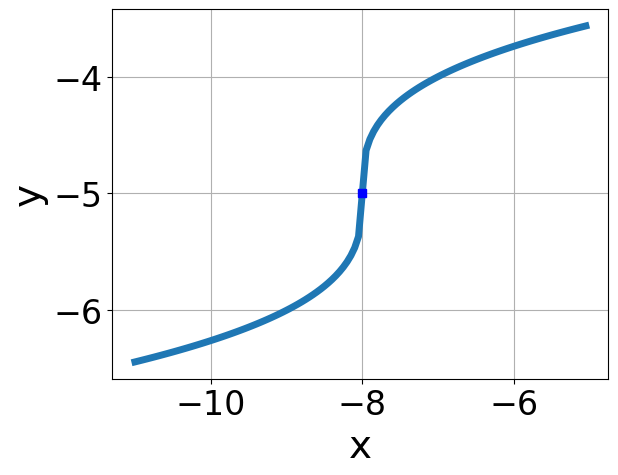
\includegraphics[width=0.5\textwidth]{../Figures/radicalGraphToEquationC.png}
\end{center}
\begin{enumerate}[label=\Alph*.]
\item \( f(x) = - \sqrt[3]{x - 8} - 5 \)
\item \( f(x) = \sqrt[3]{x - 8} - 5 \)
\item \( f(x) = \sqrt[3]{x + 8} - 5 \)
\item \( f(x) = - \sqrt[3]{x + 8} - 5 \)
\item \( \text{None of the above} \)

\end{enumerate} }
\litem{
Solve the radical equation below. Then, choose the interval(s) that the solution(s) belongs to.\[ \sqrt{-3 x - 8} - \sqrt{-4 x - 9} = 0 \]\begin{enumerate}[label=\Alph*.]
\item \( x \in [-1.8,1.1] \)
\item \( \text{All solutions lead to invalid or complex values in the equation.} \)
\item \( x \in [15.7,20.2] \)
\item \( x_1 \in [-2.8, -1.2] \text{ and } x_2 \in [-1.14,0.16] \)
\item \( x_1 \in [-2.8, -1.2] \text{ and } x_2 \in [-2.82,-1.26] \)

\end{enumerate} }
\litem{
What is the domain of the function below?\[ f(x) = \sqrt[7]{-6 x - 7} \]\begin{enumerate}[label=\Alph*.]
\item \( \text{The domain is } [a, \infty), \text{   where } a \in [-1.04, -0.21] \)
\item \( \text{The domain is } (-\infty, a], \text{   where } a \in [-1.77, -0.94] \)
\item \( (-\infty, \infty) \)
\item \( \text{The domain is } [a, \infty), \text{   where } a \in [-1.23, -0.91] \)
\item \( \text{The domain is } (-\infty, a], \text{   where } a \in [-1.05, -0.38] \)

\end{enumerate} }
\litem{
Choose the graph of the equation below.\[ f(x) = \sqrt[3]{x + 6} + 7 \]\begin{enumerate}[label=\Alph*.]
\begin{multicols}{2}\item 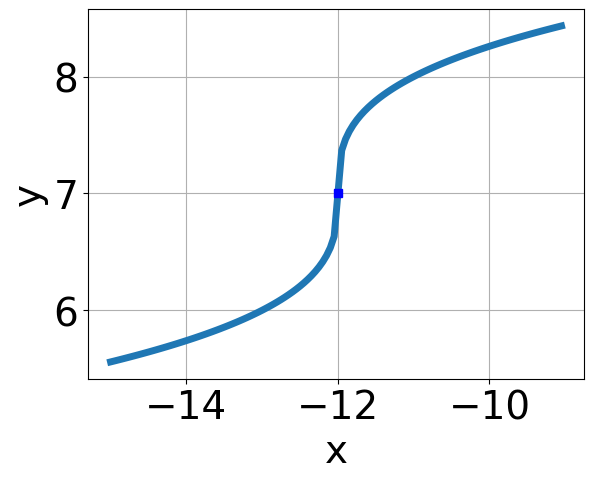
\includegraphics[width = 0.3\textwidth]{../Figures/radicalEquationToGraphCopyAC.png}\item 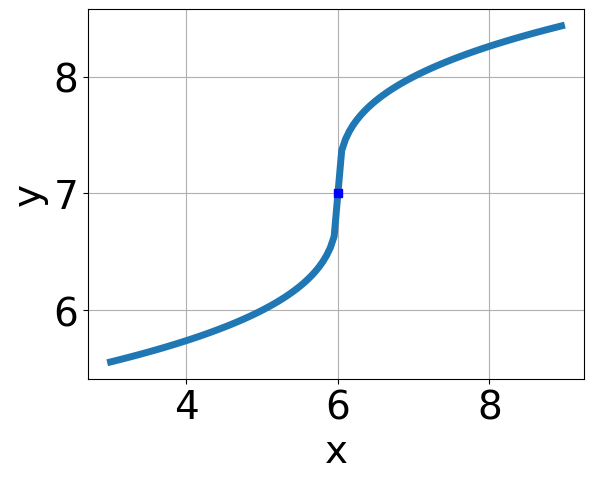
\includegraphics[width = 0.3\textwidth]{../Figures/radicalEquationToGraphCopyBC.png}\item 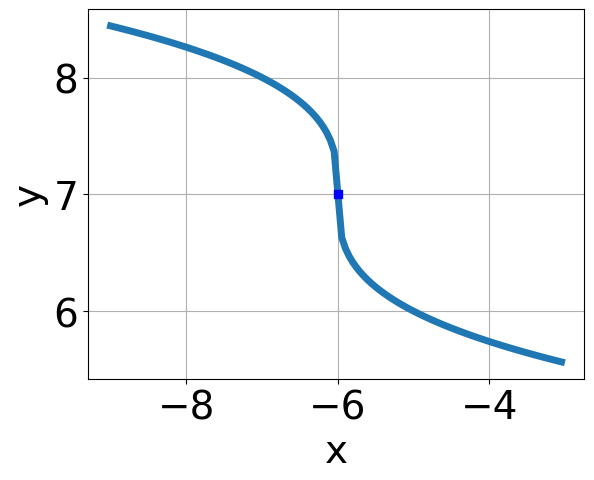
\includegraphics[width = 0.3\textwidth]{../Figures/radicalEquationToGraphCopyCC.png}\item 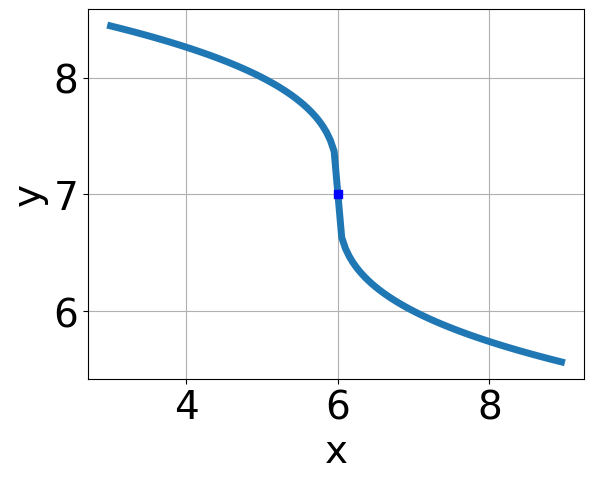
\includegraphics[width = 0.3\textwidth]{../Figures/radicalEquationToGraphCopyDC.png}\end{multicols}\item None of the above.
\end{enumerate} }
\litem{
Choose the equation of the function graphed below.
\begin{center}
    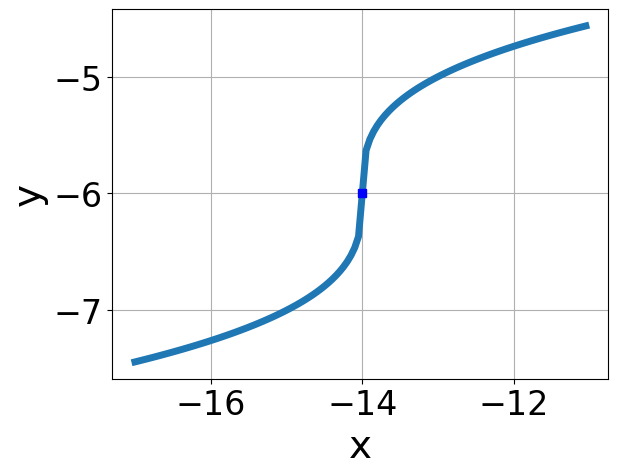
\includegraphics[width=0.5\textwidth]{../Figures/radicalGraphToEquationCopyC.png}
\end{center}
\begin{enumerate}[label=\Alph*.]
\item \( f(x) = \sqrt[3]{x - 14} - 6 \)
\item \( f(x) = - \sqrt[3]{x + 14} - 6 \)
\item \( f(x) = - \sqrt[3]{x - 14} - 6 \)
\item \( f(x) = \sqrt[3]{x + 14} - 6 \)
\item \( \text{None of the above} \)

\end{enumerate} }
\litem{
Solve the radical equation below. Then, choose the interval(s) that the solution(s) belongs to.\[ \sqrt{56 x^2 + 54} - \sqrt{-114 x} = 0 \]\begin{enumerate}[label=\Alph*.]
\item \( x \in [-1.04,0.25] \)
\item \( x_1 \in [-1.55, -1.02] \text{ and } x_2 \in [-2,0.1] \)
\item \( x_1 \in [0.64, 2.59] \text{ and } x_2 \in [0.8,2.3] \)
\item \( x \in [-1.55,-1.02] \)
\item \( \text{All solutions lead to invalid or complex values in the equation.} \)

\end{enumerate} }
\litem{
Solve the radical equation below. Then, choose the interval(s) that the solution(s) belongs to.\[ \sqrt{-9 x^2 + 42} - \sqrt{3 x} = 0 \]\begin{enumerate}[label=\Alph*.]
\item \( x \in [1,3] \)
\item \( x \in [-5.33,-0.33] \)
\item \( x_1 \in [1, 3] \text{ and } x_2 \in [2.2,4.1] \)
\item \( \text{All solutions lead to invalid or complex values in the equation.} \)
\item \( x_1 \in [-5.33, -0.33] \text{ and } x_2 \in [0.9,2.2] \)

\end{enumerate} }
\end{enumerate}

\end{document}